\documentclass[a4paper,11pt]{article}

\usepackage[portuguese]{babel}
\usepackage[utf8]{inputenc}
\usepackage[charter]{mathdesign} % charter or utopia?
\usepackage{multirow}
\usepackage[pdftex]{hyperref}
\usepackage{indentfirst}
\usepackage{xspace}
\usepackage[cm]{fullpage}
\usepackage{color, colortbl}
\usepackage{graphicx}
\usepackage{multirow}
\usepackage{fancyhdr}
\usepackage{tabu}
\usepackage{todonotes}
\usepackage[acronym,nowarn]{glossaries}
\newacronym{ASYNC}{ASYNC}{\textit{MPPA Asynchronous Communication}}
\newcommand{\async}{\gls{ASYNC}\xspace}

\newacronym{MPI}{MPI}{\textit{Message Passing Interface}}
\newcommand{\mpi}{\gls{MPI}\xspace}

\newacronym{openMP}{OpenMP}{\textit{Open Multi-Processing}}
    \newcommand{\openMP}{\gls{openMP}\xspace}

\newacronym{api}{API}{\textit{Application Programming Interface}}
    \newcommand{\api}{\gls{api}\xspace}
    \newcommand{\apis}{\glspl{api}\xspace}
    
\newacronym{hpc}{HPC}{computação de alto desempenho}
	\newcommand{\hpc}{\gls{hpc}\xspace}
	
\newacronym{cpu}{CPU}{\textit{Central Processing Unit}}
    \newcommand{\cpu}{\gls{cpu}\xspace}

    \newacronym{cpus}{CPUs}{\textit{Central Processing Units}}
    \newcommand{\cpus}{\gls{cpus}\xspace}

\newacronym{flops}{Flops}{\textit{Floating-point Operations per Second}}
    \newcommand{\flops}{\gls{flops}\xspace}

\newacronym{cnoc}{C-NoC}{\textit{Control NoC}}
    \newcommand{\cnoc}{\gls{cnoc}\xspace}

\newacronym{dnoc}{D-NoC}{\textit{Data NoC}}
    \newcommand{\dnoc}{\gls{dnoc}\xspace}

\newacronym{mpsoc}{MPSoC}{\textit{Multiprocessor System-on-Chip}}
    \newcommand{\mpsoc}{\gls{mpsoc}\xspace}

\newacronym{noc}{NoC}{\textit{Network-on-Chip}}
    \newcommand{\noc}{\gls{noc}\xspace}
    \newcommand{\nocs}{\glspl{noc}\xspace}

\newacronym{pe}{PE}{\textit{Processing Element}}
    \newcommand{\pe}{\gls{pe}\xspace}
    \newcommand{\pes}{\glspl{pe}\xspace}

\newacronym{rm}{RM}{\textit{Resource Manager}}
    \newcommand{\rman}{\gls{rm}\xspace}
    \newcommand{\rmans}{\glspl{rm}\xspace}

\newacronym{smp}{SMP}{\textit{Symmetric Multiprocessing}}
    \newcommand{\smp}{\gls{smp}\xspace}

\newacronym{spmd}{SPMD}{\textit{Single Program, Multiple Data}}
    \newcommand{\spmd}{\gls{spmd}\xspace}

    \newacronym{simd}{SIMD}{\textit{Single Instruction, Multiple Data}}
    \newcommand{\simd}{\gls{simd}\xspace}

\newacronym{vliw}{VLIW}{\textit{Very Long Instruction Word}}
    \newcommand{\vliw}{\gls{vliw}\xspace}

\newacronym{gpu}{GPU}{\textit{Graphics Processing Unit}}
    \newcommand{\gpu}{\gls{gpu}\xspace}
    \newcommand{\gpus}{\glspl{gpu}\xspace}

\newacronym{rapl}{RAPL}{\textit{Running Average Power Limit}}
    \newcommand{\rapl}{\gls{rapl}\xspace}

\newacronym{lpddr}{LPDDR3}{\textit{Low Power Double Data Rate 3}}
    \newcommand{\lpddr}{\gls{lpddr}\xspace}

\newacronym{io}{E/S}{Entrada e Saída}
    \newcommand{\io}{\gls{io}\xspace}
   
\newacronym{cc}{CC}{\textit{cluster} de computação}
	\newcommand{\cc}{\gls{cc}\xspace}

\newacronym{ccs}{CCs}{\textit{clusters} de computação}
	\newcommand{\ccs}{\gls{ccs}\xspace}

\newacronym{ipc}{IPC}{\textit{Inter-Process Communication}}
   \newcommand{\ipc}{\gls{ipc}\xspace}

\newacronym{numa}{NUMA}{\textit{Non-Uniform Memory Access}}
	\newcommand{\numa}{\gls{numa}\xspace}

\newacronym{ccnuma}{CC-NUMA}{\textit{Cache-Coherent Non-Uniform Memory Access}}
\newcommand{\ccnuma}{\gls{ccnuma}\xspace}

\newacronym{ncnuma}{NC-NUMA}{\textit{No Cache Non-Uniform Memory Access}}
\newcommand{\ncnuma}{\gls{ncnuma}\xspace}

\newacronym{soc}{SoC}{\textit{System-on-Chip}}
\newcommand{\soc}{\gls{soc}\xspace}

\newacronym{cmp}{CMP}{\textit{Chip Multiprocessor}}
\newcommand{\cmp}{\gls{cmp}\xspace}

\newacronym{cmps}{CMPs}{\textit{Chip Multiprocessors}}
\newcommand{\cmps}{\gls{cmps}\xspace}


\newacronym{uma}{UMA}{\textit{Uniform Memory Access}}
    \newcommand{\uma}{\gls{uma}\xspace}

\newacronym{ram}{RAM}{\textit{Random-Access Memory}}
    \newcommand{\ram}{\gls{ram}\xspace}

\newacronym{pc}{PC}{\textit{Personal Computer}}
    \newcommand{\pc}{\gls{pc}\xspace}

\newacronym{opengl}{OpenGL}{\textit{Open Graphics Library}}
    \newcommand{\opengl}{\gls{opengl}\xspace}

\newacronym{cow}{COW}{\textit{Clusters of Workstations}}
    \newcommand{\cow}{\gls{cow}\xspace}


\newacronym{now}{NOW}{\textit{Network of Workstations}}
    \newcommand{\now}{\gls{now}\xspace}

    \newacronym{so}{SO}{\textit{Sistema Operacional}}
    \newcommand{\so}{\gls{so}\xspace}

    \newacronym{e/s}{E/S}{\textit{Entrada e Saída}}
    \newcommand{\es}{\gls{e/s}\xspace}

%    \newacronym{kb}{KB}{\textit{Kilobyte}}
%    \newcommand{\kb}{\gls{kb}\xspace}
%
%    \newacronym{mb}{MB}{\textit{Megabyte}}
%    \newcommand{\mb}{\gls{mb}\xspace}
%    
%    \newacronym{gb}{GB}{\textit{Gigabyte}}
%    \newcommand{\gb}{\gls{gb}\xspace}

    \newacronym{posix}{POSIX}{\textit{Portable Operating System Interface}}
    \newcommand{\posix}{\gls{posix}\xspace}


\makeglossaries
\usepackage{subfigure}

\newcommand{\etal}{\textit{et al}.\xspace}
\newcommand{\eg}{\textit{e.g}.,\xspace}
\newcommand{\ie}{\textit{i.e}.,\xspace}
\newcommand{\pskel}{PSkel\xspace}
\newcommand{\pskelmppa}{PSkel-MPPA\xspace}
\newcommand{\mppa}{MPPA-256\xspace}
\newcommand{\fw}{\textit{framework}\xspace}
\newcommand{\capb}{CAP Bench\xspace}
\newcommand{\epiphany}{Adapteva Epiphany\xspace}
\newcommand{\manycore}{\textit{manycore}\xspace}
\newcommand{\bench}{\textit{benchmark}\xspace}

\fancypagestyle{plain}{%
	\renewcommand{\headrulewidth}{0pt}%
	\fancyhf{}%
	\fancyhead[C]{
		\begin{tabular*}{1.012\textwidth}{l@{\extracolsep{\fill} }cr}
			\multirow{2}{*}{\hspace{-0.3cm}
\includegraphics[height=2cm, width=!]{./figs/ufsc.jpg}} & \hspace{0.8cm}Universidade Federal de Santa Catarina (UFSC) & \multirow{2}{*}{
\includegraphics[height=2cm, width=!]{./figs/ine.pdf}} \\
			& \hspace{0.8cm}Departamento de Informática e Estatística (INE) & \\
		\end{tabular*}
	}%
}

\title{\hspace{-0.6cm}\textbf{Relatório Final - PIBIC 2018/2019}\\[0.2cm] \hspace{-0.6cm}\textbf{Projeto:} Otimização do Benchmark \capb para o Processador Manycore de Baixo Consumo Energético \mppa}
\author{\hspace{-0.6cm}\textbf{Bolsista:} David Grunheidt Vilela Ordine\\\hspace{-0.6cm}\textbf{Orientador:} Prof. Dr. Márcio Castro\\ \hspace{-0.6cm}\small{\emph{Laboratório de Pesquisa em Sistemas Distribuídos (LaPeSD), INE/UFSC}}}
\date{\hspace{-0.6cm}\small{Florianópolis, \today}}
\begin{document}
\pagenumbering{gobble}%

\maketitle

\begin{abstract}
Similar ao que aconteceu com os processadores \textit{single-core}, ao longo de sua evolução, as tecnologias voltadas para \hpc depararam-se com uma barreia de potencia, a qual torna desvantajoso o \textit{trade-off} entre gasto energético e ganho em desempenho. Desta maneira, um novo buraco dentro desta área de pesquisa surgiu, o qual foi preenchido com o ramo de processadores \manycore de baixo consumo energético, tais quais o \mppa e o \epiphany. Devido a questões arquiteturais, como a quantidade limitada de memoria em cada \cc e o não compartilhamento de memória entre \textit{clusters}, o desafio relacionado a estes processadores e, particularmente, ao \mppa, é a implementação de aplicações que beneficiam-se totalmente do seu \textit{hardware}. Neste projeto foram propostas otimizações para as aplicações do \capb, a fim de mostrar que, apesar dos desafios, são inúmeros os benefícios da utilização do \mppa, quando implementações são feitas de modo inteligente. Os resultados mostram que o novo \textit{benchmark} superou, em desempenho, até ...x a implementação anterior. \\

\noindent\textbf{Palavras-chave}: \textit{manycores}, MPPA-256, comunicação assíncrona.
\end{abstract}

\tableofcontents

\newpage

\section{Introdução}


Para que os supercomputadores atuais consigam alcançar de forma definitiva a computação em \textit{exaescale}, é necessário que haja, de forma coesa, alto desempenho e consumo energético viável. Porém, assim como ocorreu com os avanços nas tecnologias de processadores \textit{single-core}, os quais, nas ultimas três décadas, permitiram aumento no desempenho de um processador a uma taxa anual de 40\% a 50\%  \cite{Larus:2008:TM:1364782.1364800}, a dissipação de calor nos supercomputadores que utilizam processadores do tipo \textit{multicore} chegou a um ponto que não mais permitiu a escalabilidade proporcional das variáveis citadas acima.
 
Seguindo os conceitos de \textit{Green Computing}, estudos foram realizados a fim de encontrar um \textit{trade-off} positivo entre desempenho e gasto energético, centrado na redução de gasto energético. O grande interesse da comunidade cientifica de \hpc acerca deste tema foi um dos responsáveis por alavancar a produção de novos tipos de processadores, tais quais, os \textit{manycores} de baixa potencia \mppa \cite{MPPA-2:2013}, SW26010, utilizado no supercomputador \textit{Sunway TaihuLight} \cite{sunway:2016} e o \epiphany  \cite{Olofsson2014}.

Com proposito de validar as supostas qualidades do \mppa e prover meios de comparação com outros processadores do estado da arte, \textit{Souza} \etal implementaram o \capb \cite{Castro-Souza-CCPE:2016}, \textit{benchmark} que avalia ambos desempenho e gasto energético do processador, levando em conta diversos cenários. Em sua versão inicial, utilizava uma \api de comunicaçao sincrona entre processos, denominada \ipc \cite{MPPA-2:2013}. Esta antiga \api possui alguns lados negativos, como baixo nivel de abstração e realização de sincronizações implicitas, levando a queda de desempeneho.

Neste trabalho, a fim de implementar a otimização proposta, realizou-se o porte do \capb com a nova \api de comunicação assincrona entre processos da Kalray, a \async \cite{Hascoet2017}. Esta \api possui nivel de abstração superior a \ipc, além de diferir na implementação quanto ao modelo de lógica de memória. Assim, ela simplifica a elaboração de aplicações para o \mppa, além de ganhar em desempenho e reduzir o custo energético, devido a sua caracteristica assincrona.



\subsection{Justificativa}

\begin{enumerate}

	\item \textbf{Nível aplicativo.}
		
	\item \textbf{Nível intermediário.}
	
	\item \textbf{Nível de \emph{hardware}.} 
	
\end{enumerate}

\subsection{Objetivos}

O objetivo desta pesquisa de iniciação científica é propor e implementar a otimização do \bench \capb para o processador \manycore de baixo consumo energético \mppa. Os objetivos específicos deste projeto de pesquisa estão elencados abaixo:

\begin{enumerate}
	\setlength\itemsep{0em}
	\item Investigar a viabilidade do uso do \mppa para a computação científica de alto desempenho;
	\item Estudar as \apis de comunicação existentes para o \mppa.
	\item Implementar um conjunto de aplicações paralelas para o \mppa (\bench) utilizando-se da \api \async;
	\item Avaliar os custos e benefícios do \mppa em relação ao desempenho e ao consumo de energia, assim como sua utilidade para a Computação Sustentável (\textit{Green Computing});
	\item Difundir a pesquisa e os seus resultados através de produção científica de qualidade, em periódicos e eventos relevantes na área de Processamento Paralelo e Distribuído.
\end{enumerate}

Nas seções seguintes são apresentados o desenvolvimento e os resultados produzidos, de acordo com o cronograma e as atividades propostas deste projeto de pesquisa.

\section{Revisão Bibliográfica}

Esta seção apresenta a revisão bibliográfica sobre o processador \textit{manycore} \mppa e o \textit{framework} PSkel e sua adaptação utilizada nesse trabalho. Por fim, são apresentados alguns trabalhos relacionados.

\subsection{MPPA-256}
\label{subsec:mppa}

O \mppa é um processador \textit{manycore} desenvolvido pela empresa francesa
Kalray. Esse processador possui 256 núcleos e usuário e 32 núcleos de sistema para processamento a 400 MHz. Esses núcleos estão distribuídos entre 16 \emph{clusters} de computação e 4 \emph{clusters} de \emph{Input/Output}(\io), que se comunicam através de NoCs de dados e controle. O processador utilizado no desenvolver deste projeto de pesquisa possui uma memória global de baixa potência (LPDDR3) de 2GB conectada a um dos susistemas de \io. A arquitetura do \mppa é ilustrada na Figura~\ref{fig:mppaOverall}. Cada cluster de computação tem os seguintes componentes:

\begin{itemize}
    \item 16 núcleos chamados de \emph{Processing Elements} (\pes), que são responsáveis por executar as \emph{threads} de usuário (uma \emph{thread} por \pe), e não pode ser interrompida ou preemptada;
    
    \item um \emph{Resource Manager} (\rman), responsável por executar o sistema operacional e gerenciar a comunicação;
    
    \item uma memória compartilhada de baixa latência de 2MB, que permite um grande banda e fluxo e dados e controle entre os \pes presentes no mesmo \emph{cluster} de computação; e
    
    \item dois controladores de NoC, um para dados e outro para controle.
    
\end{itemize}


\begin{figure}[t]
	\centering
	\subfigure[\mppa.]{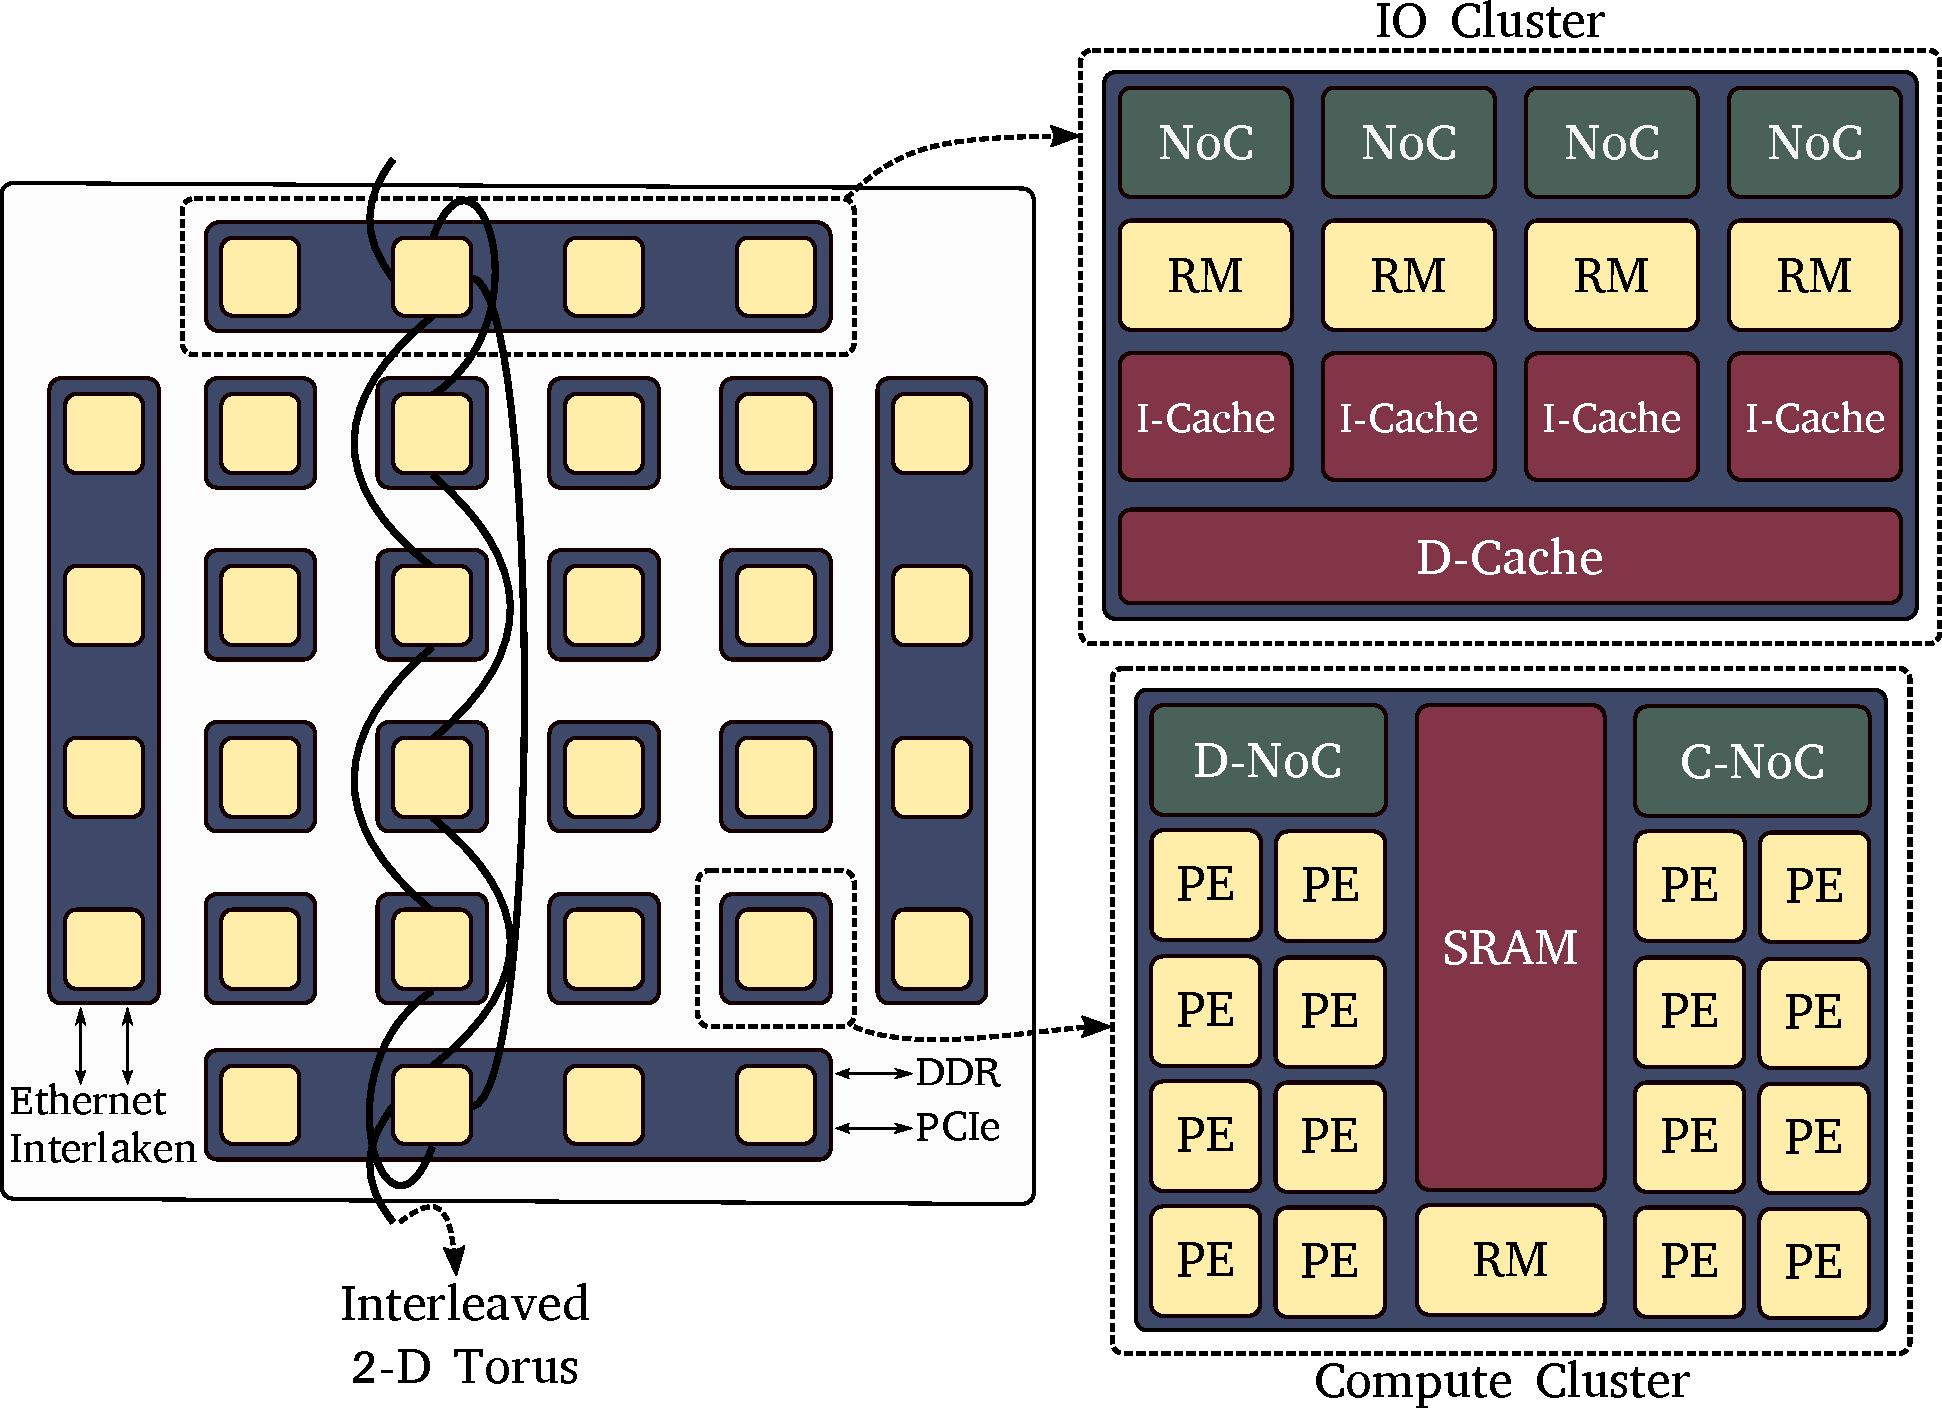
\includegraphics[width=0.3\textwidth]{figs/mppa-overview.pdf}\label{fig:mppaOverall}}
	\qquad
	\subfigure[O padrão estêncil.]{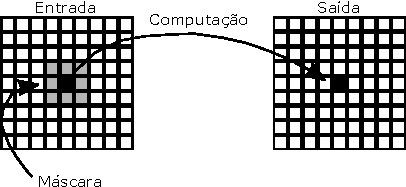
\includegraphics[width=0.38\textwidth]{figs/stencilComputation.pdf}\label{fig:stencil}}
    \caption{Visão geral do \mppa e do padrão estêncil~\cite{Castro-Podesta-ERAD:2017}.}
    \label{fig:config}
\end{figure}

Trabalhos anteriores mostraram que desenvolver aplicações paralelas otimizadas
para o \mppa é um grande desafio~\cite{Castro-IA3-JPDC:2014} devido a alguns
fatores importantes, tais como: o modelo de memória distribuída presente no
\mppa, a capacidade de memória dentro do \textit{chip} e a comunicação explícita
através da \noc. Mais detalhes sobre esses desafios são apresentados em
~\cite{Castro-Podesta-ERAD:2017}.

\subsection{Padrão estêncil e PSkel}
\label{subsec:pskel}

O \pskel é um \fw de programação em alto nível para aplicações baseadas no
padrão estêncil, baseado no conceito de esqueletos paralelos, oferecendo suporte para a execução dessas aplicações em
ambientes heterogêneos, incluindo \cpu e \gpu. \pskel oferece um interface única de programação, desacoplada do \emph{back-end} de execução, permitindo que o usuário se preocupe apenas em implementar o \emph{kernel} estêncil que descreve a computação, enquanto o \fw fica responsável pela tradução das abstrações descritas para código paralelo de baixo nível em C++, gestão de memória e transferência de dados, tudo isso de forma transparente paar o usuário~\cite{pereira15}.


\subsection{PSkel-MPPA}
\label{subsec:pskel-mppa}

A adaptação PSkel-MPPA, é uma adaptação do \pskel proposta por Podestá~\etal~\cite{PodestaJr.2017}, ela faz uso de uma \api similar à POSIX \ipc para comunicação, e será tratada como \ipc no decorrer deste relatório. Nela, são utilizados portais de comunicação para o envio de dados e o método de \textit{strides}  para gerenciar explicitamente o envio e recebimento de \textit{tiles}. Essa adaptação possíbilita o uso do \fw PSkel com o processador \emph{manycore} \mppa.

\subsection{Trabalhos Relacionados}

Devido a importância dos esqueletos paralelos, e especifcamente o padrão paralelo estêncil, muitos esforços de pesquisas recentes buscam melhorar o desempenho e o suporte desses esqueletos em processadores manycore. \emph{Buono}~\etal~\cite{buono13} portou um \fw baseado em esqueletos paralelos, chamado \emph{FastFlow}, para o processador \emph{manycore} TilePro64, que possui 64 núcleos de processamento idênticos, interconectados por uma malha de \noc. Similarmente, \emph{Thorarensen}~\etal~\cite{thoraransen16} apresentou um novo \emph{back-end} do \fw SkePU para o processador \emph{manycore} Myriad2. Que possui como característica uma arquitetura heterogenea, visando dispositivos com restrição de energia e principalmente aplicações de visão computacional. \emph{Gysi}~\etal~\cite{gysi15} propôs um \fw para otimização automática da repartição de computações estêncil em sistemas híbridos de \cpu e \gpu.

Recentes trabalhos estudaram o desempenho e/ou a eficiência energética de processadores manycore de baixa potência. \emph{Totoni}~\etal~\cite{SCCEnergy:2012} comparou a potência e o desempenho do \emph{Intel's Single-Chip Cloud Computer} (SCC) com outros tipos de \emph{CPUs} e \emph{GPUs}. Porém, eles mostraram que não existe um solução única que entrega o melhor troca entre potência e performance, os resultados mostram que \emph{manycores} são uma oportunidade para o futuro. \emph{Souza}~\etal~\cite{Castro-Souza-CCPE:2016} propôs um conjunto de \emph{benchmarks} para avaliar o \mppa manycore processor. O \emph{benchmark} oferece diversas aplicações que utilizam padrões paralelos, tipos de trabalho, intensidade de comunicação e estratégias de carga de trabalho, adequado para uma ampla compreensão do desempenho e consumo de energia do \mppa e novos \emph{manycores} que estão por vir. \emph{Francesquini}~\etal~\cite{Castro-IA3-JPDC:2014} avaliou três diferentes classes de aplicação (consumo de CPU, consumo de memória e uma composição híbrida dos dois tipos anteriores) utilizando plataformas de alto paralelismo como o \mppa em uma plataforma NUMA de 24 nós e 192 núcleos. Eles mostraram que as arquiteturas \emph{manycore} podem ser competitivas, mesmo se a aplicação é irregular por natureza.

De acordo com relevante conhecimento na área, o \pskelmppa é a primeira implementação completa de um \fw com uso de padrões paralelos no \mppa. A solução proposta livra os programadores da necessidade de lidar explicitamente com a gestão de comunicação e envio de dados pela \noc, assim como a preocupação de lidar com um ambiente híbrido de execução e a ausência de coerência de cache no \mppa.

\section{Proposta e implementação de otimização no PSkel-MPPA}
\label{sec:pskelMPPA}

As otimizações propostas e implementação das mesmas continua aplicando o modelo mestre-trabalhador, que é um dos padrões de computação paralela que pode ser utilizado quando existem múltiplos núcleos de processamento. O processo mestre é executado no \emph{cluster} de \io conectado a memória LPDDR3, aonde os dados de entrada e saída (os \emph{Array2Ds}) são alocados, enquanto os processos dos trabalhadores são executados nos \emph{clusters} de computação (um processo trabalhador por \emph{cluster} de computação) para realizar a computação estêncil. Devido a memória limitada nos \emph{clusters} de computação (2MB), o tamanho do \emph{Array2D} é particionado em \emph{tiles} de tamanho fixo definido pelo usuário para serem enviados à eles. Quando se trata de particionamento de computação estêncil, é necessário tratar as depedências de vizinhança provenientes do padrão paralelo estêncil, antes de particionar os dados de entrada.


\begin{figure}[htb]
  \begin{minipage}[b]{0.40\textwidth}
	\centering
	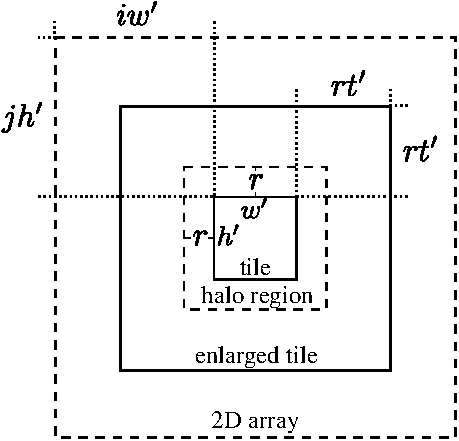
\includegraphics[height=3.8cm]{figs/tile.pdf}
	\caption{Técnica de \emph{tiling} 2D~\cite{Rocha:2017}.}
	\label{fig:gputile}
  \end{minipage}
  \begin{minipage}[b]{0.60\textwidth}
	\centering
	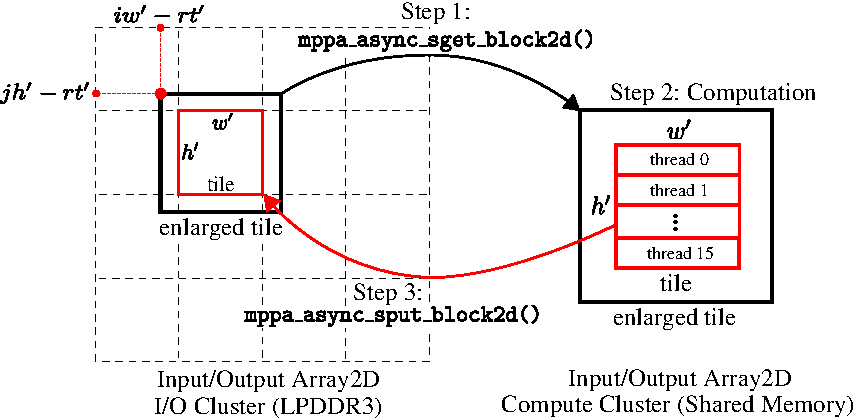
\includegraphics[height=3.8cm]{figs/pskel-mppa-fluxogram.pdf}
	\caption{Comunicações com \texttt{block2d}.}
    \label{fig:block2d}
  \end{minipage}
\end{figure}

O fluxo de execução do \pskelmppa ocorre da seguinte forma. Durante a fase de inicialização, o processo mestre que está executando no \emph{cluster} de \io aloca os dados de entrada e saída na \lpddr, e cria um segmento específico para cada uma deles. Em seguida, ele calcula o número de \emph{tiles} engordados que serão produzidos assim como suas dimensões baseado em: i) parametros definidos pelo usuário, como o tamanho da entrada de dados e as dimensões do \emph{tile} lógico, o número de \emph{clusters} de computação e o número de iterações internas; e ii) parâmetros do \emph{kernel} estêncil, como o tamanho da máscara. Então, são lançados até 16 processos trabalhadores (um em cada \emph{cluster} de computação) e é informado a cada processo trabalhador o número de \emph{tiles} engordados gerados, suas dimensões e o subconjunto de \emph{tiles} que cada \emph{cluster} será responsável por processar. Por fim, o processo mestre aguarda até que todos os trabalhadores terminem de computar.
%
Cada processo trabalhador, por outro lado, aloca dados para armazenar os \emph{tiles} engordados de entrada e de saída na memória local do \emph{cluster} de computação e clona ambos os segmentos de entrada e saída que foram criados pelo processo mestre para realizar futuras transferências de dados. A fase de inicialização tanto do mestre como do trabalhor está encapsulada na classe \texttt{Stencil2D}.
%
Essa primeira etapa do fluxo de execução diferencia-se da anteriormente presente no PSkelMPPA, pois agora esta comunicação é realizada uma única vez na inicialização, o que não ocorria anteriormente, já que exisitiam trocas de mensagens de sincronização a cada laço da computação iterativa.

As etapas acima mencionadas estão retratadas na Figura~\ref{fig:block2d}, para sua implementação foi utilizada uma nova \api de comunicação asíncrona (ASYNC) disponível para o \mppa, que difere da \api anteriormente utilizada, a \ipc. Abaixo elas são descritas em mais detalhes:

\begin{description}




	\item[Etapa 3.] Após a computação do \emph{kernel} estêncil, o\emph{tile} lógico resultante é transferido de volta para a \lpddr. A função \texttt{mppa\_async\_sput\_block2d()} é usada para esse propósito, permitindo que o \emph{tile} lógico seja extraído do \emph{tile} engordado na memória local do \emph{cluster} de computação e seja transferido para sua posicão correspondente no segmento de saída remoto.

\end{description}

Felizmente, todas a complexas tarefas relacionas a técnica de \emph{tiling}, comunicação via \noc e adaptações discutidas nessa seção são transparentes para os desenvolvedores, tendo em vista que estão incluidas no \emph{back-end} do PSkelMPPA. Isso significa que aplicações desenvolvidas com o \fw PSkel podem executar perfeitamente no \mppa sem nenhuma alteração no seu código fonte.

\section{Resultados}
\label{sec:resultados}

Esta seção apresenta os resultados obtidos com a solução proposta, comparando-a com a versão apresentada em~\cite{PodestaJr.2017}.
Todas as métricas foram obtidas com auxílio de ferramentas disponíveis no \mppa.
Os dados se referem a execução de uma única iteração das aplicações Fur, GoL e Jacobi.
A aplicação \textbf{\textit{Fur}} realiza a simulação de padrões de pigmento sobre
pelos de animais. A aplicação \textbf{\textit{GoL}} é um autômato celular que
implementa o Jogo da Vida de Conway. Por fim, a aplicação
\textbf{\textit{Jacobi}} implementa o método de Jacobi para a resolução de equações matriciais.

A variabilidade dos valores obtidos foi extremamente pequena (desvio-padrão inferior à $1\%$), pois as \textit{threads} da aplicação são executadas de maneira ininterrupta no \mppa.

\begin{figure}[t]
	\centering
	\subfigure[Escalabilidade.]{
		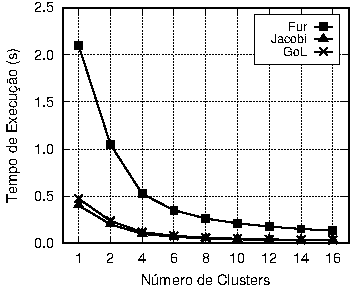
\includegraphics[width=0.3\textwidth]{figs/MPPAPlotScalabilityAPI.pdf}
		\label{fig:escalabilidade}
	}
%	\quad
	\subfigure[\textit{Tiles} vs. tempo (Fur).]{
		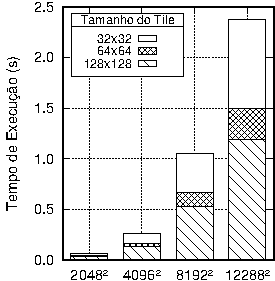
\includegraphics[width=0.242\textwidth]{figs/MPPAPlotAPIfurTimeTiles.pdf}
		\label{fig:tiles}
	}
%	\quad
	\subfigure[Tempo.]{
		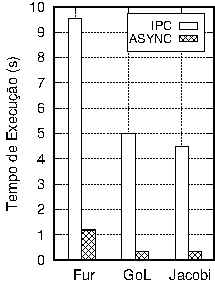
\includegraphics[width=0.19\textwidth]{figs/ComparisonTimeTiles1.pdf}
		\label{fig:compara-tempo}
	}
%	\quad
	\subfigure[Energia.]{
		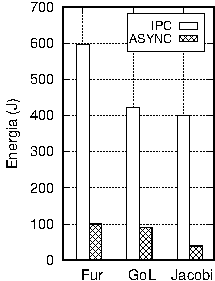
\includegraphics[width=0.19\textwidth]{figs/ComparisonEnergyTiles1.pdf}
		\label{fig:compara-energia}
	}
    \caption{Escalabilidade (a) e impacto do tamanho dos \textit{tiles} (b) na versão ASYNC. Comparação do tempo (c) e consumo de energia (d) do ASYNC com a versão IPC.}
    \label{fig:compara}
\end{figure}

\section{Conclusão}
\label{sec:conclusao}



\section{Avaliação PIBIC: Benefícios e Formação Científica}

Este projeto de pesquisa contribuiu de inumeras formas para minha formação academica. Do começo ao fim foi algo engrandecedor e acredito que, ao longo da minha carreira profissional, irei utilizar diversos conhecimentos aqui adquiridos. Este foi o primeiro projeto no qual tive contato com uma documentação de \api, e, assim como nosso primeiro contato com qualquer tecnologia nova, foi bastante desafiador. Através de muita dedicação e ajuda do meu orientador e colegas de trabalho, consegui quebrar as barreiras do conhecimento e entender a fundo como funciona a nova \api da Kalray, a \async.  

Neste ciclo de pesquisa também produzi um artigo científico, o qual foi aprovado na decima nona Escola Regional de Alto Desempenho da Região Sul (ERAD/RS 2019), ocorrida na cidade de Três de Maio, no Rio Grande do Sul. Com esta aprovação, fui apresenta-lo nesta mesma cidade na data de realização do evento. Participar deste evento foi também uma experiencia enriquecedora, pois pude conhecer projetos de diferentes niveis de complexidade, engloblando tanto projetos de iniciação ciêntifica quanto os do estado da arte.

Com este projeto de pesquisa pude também descobrir o que pretendo seguir na minha carreia profissional, assim como ter plena certeza de que de quero continuar com a pesquisa e contribuir de forma significativa para o avanço tecnologico de toda comunidade cientifica. Utiliarei também os resultados deste para realização do meu trabalho de conclusão de curso, onde pretendo expandir o que já foi pesquisado, realizando comparações com outros processadores do estado da arte.
 
\bibliography{bibliografia} 
\bibliographystyle{sbc}

\end{document}
